% !TEX TS-program = pdflatex
% !TEX encoding = UTF-8 Unicode

% This file is a template using the "beamer" package to create slides for a talk or presentation
% - Talk at a conference/colloquium.
% - Talk length is about 20min.
% - Style is ornate.

% MODIFIED by Jonathan Kew, 2008-07-06
% The header comments and encoding in this file were modified for inclusion with TeXworks.
% The content is otherwise unchanged from the original distributed with the beamer package.

\documentclass{beamer}


% Copyright 2004 by Till Tantau <tantau@users.sourceforge.net>.
%
% In principle, this file can be redistributed and/or modified under
% the terms of the GNU Public License, version 2.
%
% However, this file is supposed to be a template to be modified
% for your own needs. For this reason, if you use this file as a
% template and not specifically distribute it as part of a another
% package/program, I grant the extra permission to freely copy and
% modify this file as you see fit and even to delete this copyright
% notice. 


\mode<presentation>
{
  \usetheme{Warsaw}
  % or ...

  \setbeamercovered{transparent}
  % or whatever (possibly just delete it)
}


\usepackage{graphicx}
\usepackage[english]{babel}
\usepackage[utf8]{inputenc}
\usepackage{times}
\usepackage[T1]{fontenc}
% Or whatever. Note that the encoding and the font should match. If T1
% does not look nice, try deleting the line with the fontenc.

\setbeamertemplate{navigation symbols}{}%remove navigation symbols

\logo{
\includegraphics[height=1cm]{ideaisMinColor.png}}

%\institute[My Institute/company]{My Institute/company\\ \pgfdeclareimage[height=0.5cm]{myalias}{pselogo} %declare logo image with an alias here \pgfuseimage{myalias}} %use the image right after

\title[Short Paper Title] % (optional, use only with long paper titles)
{Title As It Is In the Proceedings}

\subtitle
{Include Only If Paper Has a Subtitle}

\author[Author, Another] % (optional, use only with lots of authors)
{F.~Author\inst{1} \and S.~Another\inst{2}}
% - Give the names in the same order as the appear in the paper.
% - Use the \inst{?} command only if the authors have different
%   affiliation.

\institute[Universities of Somewhere and Elsewhere] % (optional, but mostly needed)
{
  \inst{1}%
  Department of Computer Science\\
  University of Somewhere\\
  
\includegraphics[height=1cm]{ideaisMinColor.png}
  \and
  \inst{2}%
  Department of Theoretical Philosophy\\
  University of Elsewhere
}
% - Use the \inst command only if there are several affiliations.
% - Keep it simple, no one is interested in your street address.

\date[CFP 2003] % (optional, should be abbreviation of conference name)
{Conference on Fabulous Presentations, 2003}
% - Either use conference name or its abbreviation.
% - Not really informative to the audience, more for people (including
%   yourself) who are reading the slides online

\subject{Theoretical Computer Science}
% This is only inserted into the PDF information catalog. Can be left
% out. 

% If you have a file called "university-logo-filename.xxx", where xxx
% is a graphic format that can be processed by latex or pdflatex,
% resp., then you can add a logo as follows:

% \pgfdeclareimage[height=0.5cm]{university-logo}{university-logo-filename}
% \logo{\pgfuseimage{university-logo}}

% Delete this, if you do not want the table of contents to pop up at
% the beginning of each subsection:
\AtBeginSubsection[]
{
  \begin{frame}<beamer>{Outline}
    \tableofcontents[currentsection,currentsubsection]
  \end{frame}
}


% If you wish to uncover everything in a step-wise fashion, uncomment
% the following command: 

%\beamerdefaultoverlayspecification{<+->}

\begin{document}

\begin{frame}
  \titlepage
\end{frame}

\begin{frame}{Outline}
  \tableofcontents[pausesections]
  % You might wish to add the option [pausesections]
\end{frame}


% Structuring a talk is a difficult task and the following structure
% may not be suitable. Here are some rules that apply for this
% solution: 

% - Exactly two or three sections (other than the summary).
% - At *most* three subsections per section.
% - Talk about 30s to 2min per frame. So there should be between about
%   15 and 30 frames, all told.

% - A conference audience is likely to know very little of what you
%   are going to talk about. So *simplify*!
% - In a 20min talk, getting the main ideas across is hard
%   enough. Leave out details, even if it means being less precise than
%   you think necessary.
% - If you omit details that are vital to the proof/implementation,
%   just say so once. Everybody will be happy with that.

\section{Motivation}

\subsection{The Basic Problem That We Studied}

\begin{frame}
	\frametitle{`Hidden higher-order concepts?'}
	\begin{itemize}[<+->]
	\item The truths of arithmetic which are independent of PA in some 
	sense themselves `{contain} essentially {\color{blue}{hidden higher-order}},
	 or infinitary, concepts'???
	\item `Truths in the language of arithmetic which \ldots
	\item	That suggests stronger version of Isaacson's thesis. 
	\end{itemize}
\end{frame}

\begin{frame}{Columns}
    \begin{columns}[c] % the "c" option specifies center vertical alignment
    \column{.5\textwidth} % column designated by a command
     Contents of the first column
    \column{.5\textwidth}
     Contents split \\ into two lines
    \end{columns}
\end{frame}
 
\begin{frame}{Columns and Alignment}
     \begin{columns}[t] % contents are top vertically aligned
     \begin{column}[T]{5cm} % each column can also be its own environment
     Contents of first column \\ split into two lines
     \end{column}
     \begin{column}[T]{5cm} % alternative top-align that's better for graphics
         % \includegraphics[height=3cm]{graphic.png}
	Contents of second column with bigger line to see how break works
     \end{column}
     \end{columns}
\end{frame}

\begin{frame}{Blocks}
 
   \begin{block}{This is a Block}
      This is important information
   \end{block}
 
   \begin{alertblock}{This is an Alert block}
   This is an important alert
   \end{alertblock}
 
   \begin{exampleblock}{This is an Example block}
   This is an example 
   \end{exampleblock}
 
\end{frame}

\begin{frame}{Images}
 
    \centering{ 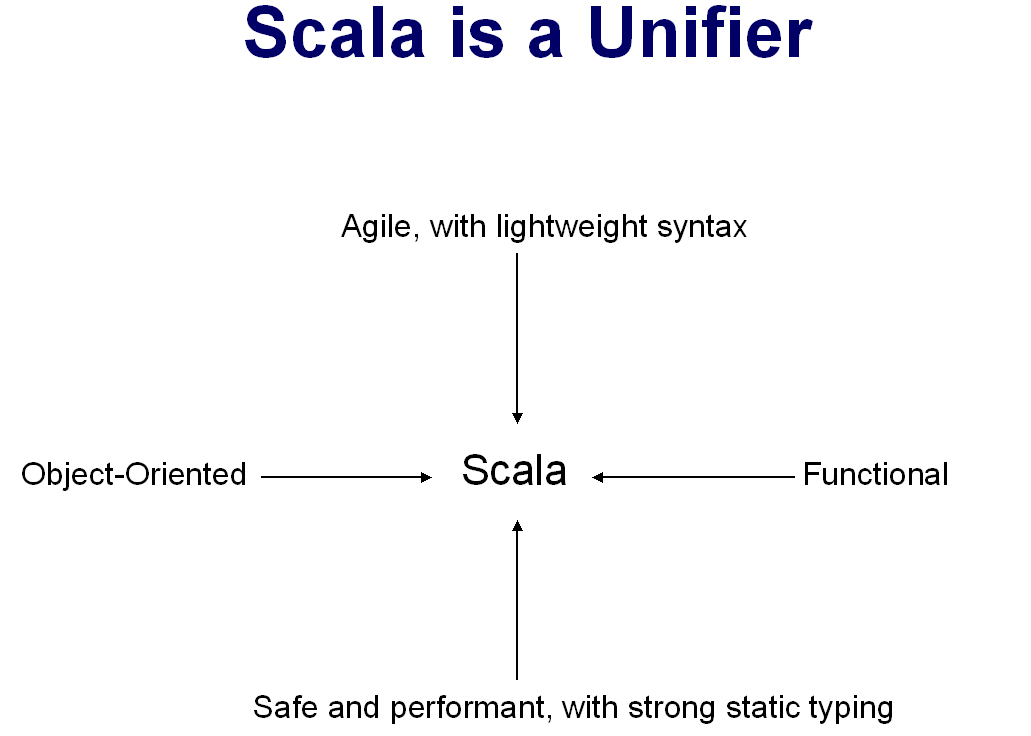
\includegraphics[scale=0.20]{Scala-is-a-Unifier.png}   }
 
\end{frame}



\begin{frame}{Make Titles Informative. Use Uppercase Letters.}{Subtitles are optional.}
  % - A title should summarize the slide in an understandable fashion
  %   for anyone how does not follow everything on the slide itself.

  \begin{itemize}
  \item
    Use \texttt{itemize} a lot.
  \item
    Use very short sentences or short phrases.
  \end{itemize}
\end{frame}

\begin{frame}{Make Titles Informative.}

  You can create overlays\dots
  \begin{itemize}
  \item using the \texttt{pause} command:
    \begin{itemize}
    \item
      First item.
      \pause
    \item    
      Second item.
    \end{itemize}
  \item
    using overlay specifications:
    \begin{itemize}
    \item<3->
      First item.
    \item<4->
      Second item.
    \end{itemize}
  \item
    using the general \texttt{uncover} command:
    \begin{itemize}
      \uncover<5->{\item
        First item.}
      \uncover<6->{\item
        Second item.}
    \end{itemize}
  \end{itemize}
\end{frame}


\subsection{Previous Work}

\begin{frame}{Make Titles Informative.}
\end{frame}

\begin{frame}{Make Titles Informative.}
\end{frame}



\section{Our Results/Contribution}

\subsection{Main Results}

\begin{frame}{Make Titles Informative.}
\end{frame}

\begin{frame}{Make Titles Informative.}
\end{frame}

\begin{frame}{Make Titles Informative.}
\end{frame}


\subsection{Basic Ideas for Proofs/Implementation}

\begin{frame}{Make Titles Informative.}
\end{frame}

\begin{frame}{Make Titles Informative.}
\end{frame}

\begin{frame}{Make Titles Informative.}
\end{frame}



\section*{Summary}

\begin{frame}{Summary}

  % Keep the summary *very short*.
  \begin{itemize}
  \item
    The \alert{first main message} of your talk in one or two lines.
  \item
    The \alert{second main message} of your talk in one or two lines.
  \item
    Perhaps a \alert{third message}, but not more than that.
  \end{itemize}
  
  % The following outlook is optional.
  \vskip0pt plus.5fill
  \begin{itemize}
  \item
    Outlook
    \begin{itemize}
    \item
      Something you haven't solved.
    \item
      Something else you haven't solved.
    \end{itemize}
  \end{itemize}
\end{frame}



% All of the following is optional and typically not needed. 
\appendix
\section<presentation>*{\appendixname}
\subsection<presentation>*{For Further Reading}

\begin{frame}[allowframebreaks]
  \frametitle<presentation>{For Further Reading}
    
  \begin{thebibliography}{10}
    
  \beamertemplatebookbibitems
  % Start with overview books.

  \bibitem{Author1990}
    A.~Author.
    \newblock {\em Handbook of Everything}.
    \newblock Some Press, 1990.
 
    
  \beamertemplatearticlebibitems
  % Followed by interesting articles. Keep the list short. 

  \bibitem{Someone2000}
    S.~Someone.
    \newblock On this and that.
    \newblock {\em Journal of This and That}, 2(1):50--100,
    2000.
  \end{thebibliography}
\end{frame}

\end{document}


